\documentclass[tikz,border=24pt]{standalone}
\usepackage{tikz}
% Use cleaner arrow tips and calc utilities
\usetikzlibrary{positioning,arrows.meta,calc,shadows}

\begin{document}
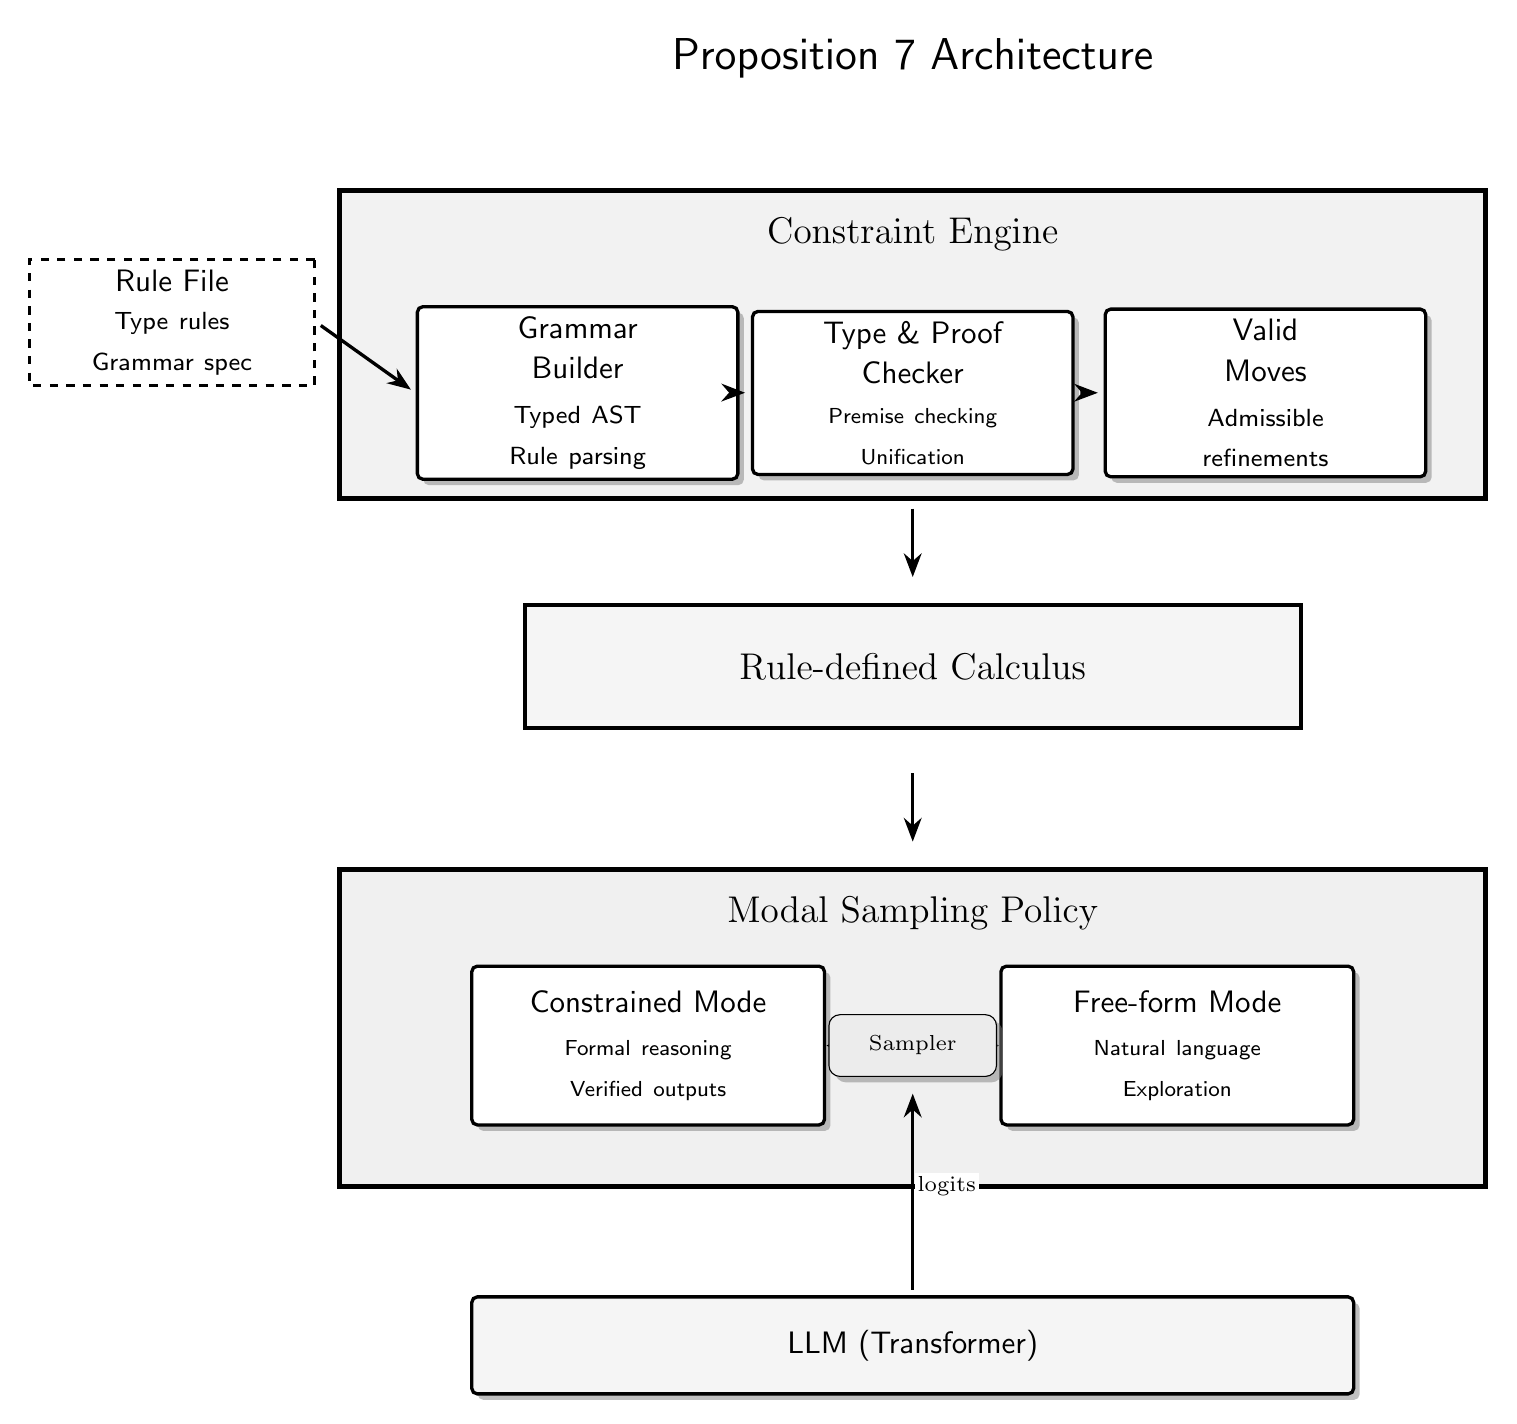
\begin{tikzpicture}[
    scale=1.12, transform shape,
    node distance=0.8cm,
    every node/.style={font=\sffamily},
    box/.style={rectangle, rounded corners=2pt, draw=black, line width=1.2pt, fill=white, drop shadow, minimum width=3.6cm, minimum height=1.5cm, align=center, text width=3.4cm},
    bigbox/.style={rectangle, draw=black, line width=1.6pt, minimum width=13cm, align=center},
    inputbox/.style={rectangle, draw=black, dashed, line width=1.2pt, minimum width=3.2cm, minimum height=1.2cm, align=center, text width=3cm},
    arrow/.style={->, >={Stealth[length=3mm]}, line width=1.2pt, shorten <= 2pt, shorten >= 2pt}
]

% Title
\node[font=\Large\sffamily] (title) at (0,11) {Proposition 7 Architecture};

% Rule File Input
\node[inputbox, minimum width=2.8cm] (rulefile) at (-8.4,8) {Rule File\\[3pt]\footnotesize Type rules\\[1pt]\footnotesize Grammar spec};

% Constraint Engine outer box (grayscale)
\draw[line width=1.8pt, fill=gray!10] (-6.5,6) rectangle (6.5,9.5);
\node[font=\large] at (0,9) {Constraint Engine};

% Components inside Constraint Engine
\node[box] (grammar) at (-3.8,7.2) {Grammar\\[1pt]Builder\\[5pt]\footnotesize Typed AST\\[1pt]\footnotesize Rule parsing};

\node[box] (checker) at (0,7.2) {Type \& Proof\\[1pt]Checker\\[5pt]\scriptsize Premise checking\\[1pt]\scriptsize Unification};

\node[box] (moves) at (4,7.2) {Valid\\[1pt]Moves\\[5pt]\footnotesize Admissible\\[1pt]\footnotesize refinements};

% Arrows within Constraint Engine
\draw[arrow] (grammar) -- (checker);
\draw[arrow] (checker) -- (moves);

% Arrow from Rule File to Grammar Builder
\draw[arrow] (rulefile.east) -- (grammar.west);

% Rule-defined Calculus (derived from rule file) — smaller box (grayscale)
\draw[line width=1.4pt, fill=gray!8] (-4.4,3.4) rectangle (4.4,4.8);
\node[font=\large] at (0,4.1) {Rule-defined Calculus};

% Arrow from Constraint Engine to Language Core
\draw[arrow] (0,5.95) -- (0,5.05);

% Modal Sampling Policy outer box (grayscale)
\draw[line width=1.8pt, fill=gray!12] (-6.5,-1.8) rectangle (6.5,1.8);
\node[font=\large] at (0,1.3) {Modal Sampling Policy};

% Constrained Mode
\node[box, minimum height=1.8cm, minimum width=4cm] (constrained) at (-3,-0.2) {
    Constrained Mode\\[6pt]
    \scriptsize Formal reasoning\\[1pt]
    \scriptsize Verified outputs
};

% Free Mode
\node[box, minimum height=1.8cm, minimum width=4cm] (free) at (3,-0.2) {
    Free-form Mode\\[6pt]
    \scriptsize Natural language\\[1pt]
    \scriptsize Exploration
};

% Midpoint between mode boxes
\path let \p1 = (constrained.east), \p2 = (free.west) in coordinate (sampler) at ($ (\p1)!0.5!(\p2) $);

% Bidirectional axis with label
\draw[<->, >=stealth, thick] (constrained.east) -- node[above, font=\scriptsize, fill=white, inner sep=1pt] {entropy-driven} (free.west);

% Explicit sampler node at midpoint (grayscale)
\node[rectangle, rounded corners=4pt, draw=black, fill=gray!15, inner sep=4pt, minimum width=1.9cm, minimum height=0.7cm, font=\scriptsize, drop shadow] (samplernode) at (sampler) {Sampler};

% LLM below, feeding logits to the sampler
\node[rectangle, rounded corners=2pt, draw=black, line width=1.2pt, minimum width=10cm, minimum height=1.1cm, align=center, fill=gray!8, drop shadow] (llm) at (0,-3.6) {LLM (Transformer)};
% Route logits arrow to sampler border cleanly (no overlap)
\draw[arrow, shorten >= 6pt] (llm.north) -- (samplernode.south) node[midway, right, font=\scriptsize, fill=white, inner sep=1pt] {logits};

% Arrow from Language Core to Modal Sampling (stop above the box)
\draw[arrow] (0,2.95) -- (0,2.05);

\end{tikzpicture}
\end{document}
